L'obbiettivo di tutte le evoluzioni delle reti mobili è quello di migliorare le performance in termini di velocità.
Il 5G invece, si concentra su latenza, affidabilità, numero di utenti e consumo energetico.
\begin{figure}[H]
	\centering
	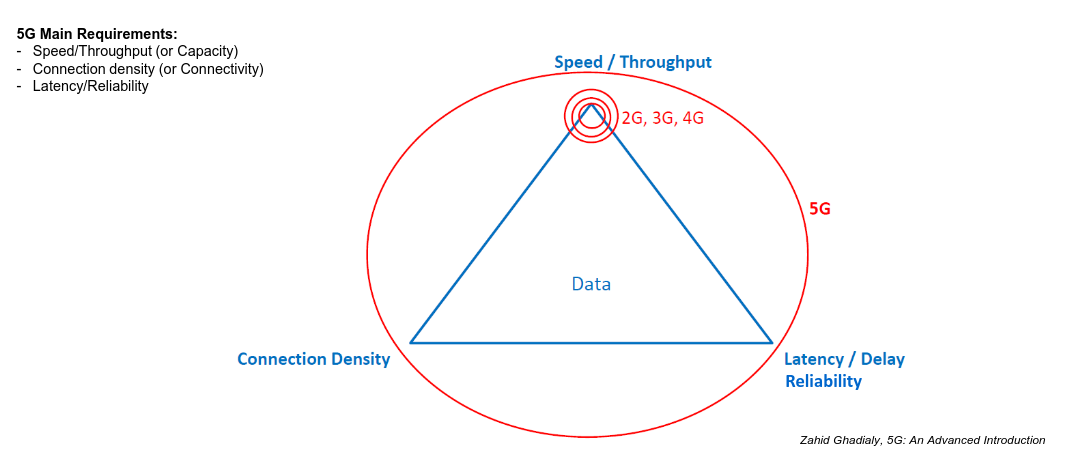
\includegraphics[width=0.9\textwidth]{pictures/12/requisiti.png}
	\caption{Requisiti del 5G}
\end{figure}	
\begin{figure}[H]
	\centering
	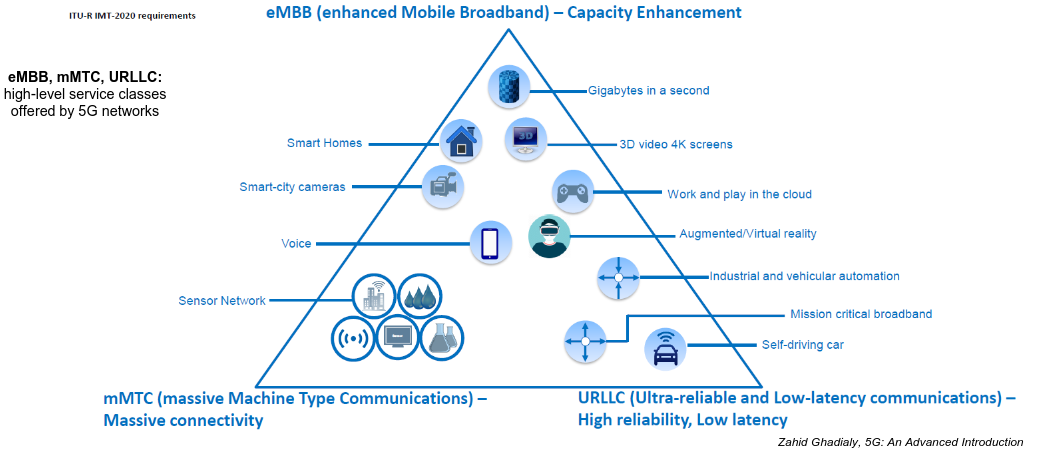
\includegraphics[width=0.9\textwidth]{pictures/12/servizi.png}
	\caption{Servizi che possono essere offerti grazie al 5G}
\end{figure}
\section{Ruolo della virtualizzazione}
La virtualizzazione ha un ruolo fondamentale nel 5G.
\subsection{Network slicing}
NFV e SDN vengono usati per la creazione di reti virtuali indipendenti, ognuna specializzata per uno scopo.
Queste reti vengono dette \textbf{slice} e vengono create dagli operatori di rete che li vendono a degli slice tenant.
\begin{figure}[H]
	\centering
	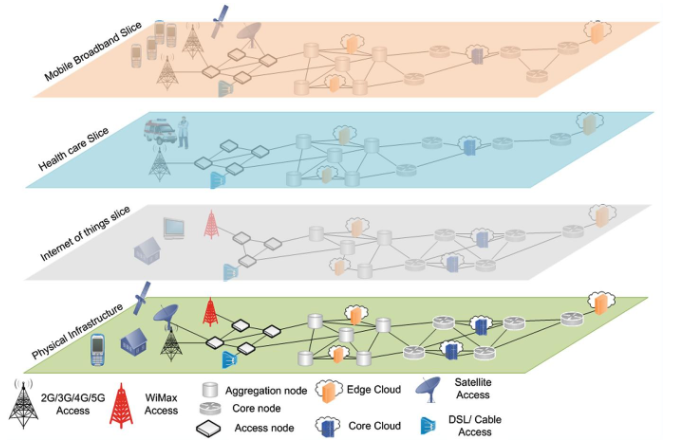
\includegraphics[width=0.75\textwidth]{pictures/12/slice.png}
	\caption{Network slicing}
\end{figure}
Lo slice tenant (ad esempio un media provider) può creare a sua volta delle reti virtuali, in modo da avere risorse dedicate e QoS specifici per i propri scopi. In questo modo inoltre, può avere una allocazione dinamica delle risorse.
Usualmente, gli slice vengono creati sia per i segmenti della RAN che il mobile core.
\begin{figure}[H]
	\centering
	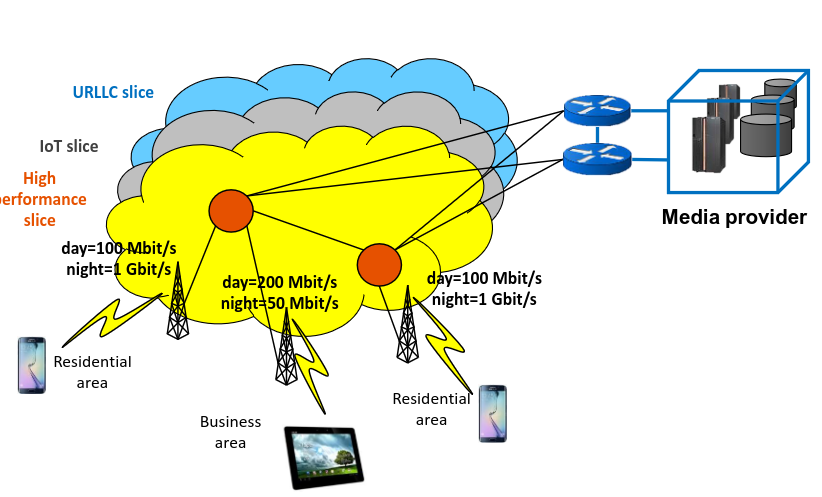
\includegraphics[width=0.8\textwidth]{pictures/12/sliceTenant.png}
	\caption{Creazione di slice da parte dello slice tenant}
\end{figure}
\subsection{Edge computing}
Risorse di memoria/calcolo/storage virtualizzate sono rese disponibili alla rete radio mobile, di solito nella RAN. Nelle reti attuali viene chiamato Multi/access Edge Computing (MEC).
La struttura della rete non serve più unicamente a trasportare i dati, ma anche a fornire capacità di calcolo sull'edge della rete (negli edge node), in modo da ridurre la latenza e offrire dei servizi innovativi.
Sia applicazioni degli utenti che servizi di rete (ad esempio sotto forma di virtual network functions) possono essere eseguiti sugli edge node.
\begin{figure}[H]
	\centering
	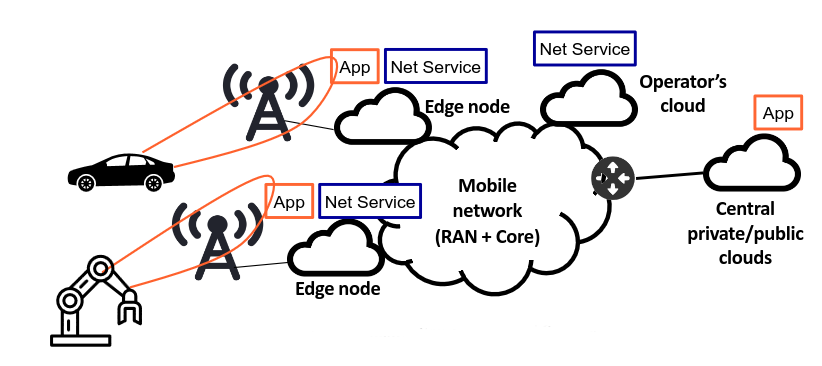
\includegraphics[width=0.8\textwidth]{pictures/12/edge.png}
	\caption{Edge computing}
\end{figure}
\section{Millimeter wave technology}
Con il termine \textbf{millimeter wave} (mmWave) si intendono le frequenze comprese tra 24 e 300 GHz, con lunghezze d'onda comprese tra 1 e 10 mm.
Questa tecnologia è molto appetibile perché quello spettro è poco usato, quindi c'è più banda disponibile e perché permette di avere antenne più piccole e quindi creare array su chip.
Le limitazioni di questa tecnologia sono:
\begin{itemize}
	\item Perdita sul percorso molto elevata, a causa delle alte frequenze.
	\item Forte attenuazione a causa della pioggia e assorbimento atmosferico.
	\item Alto blocco da parte di oggetti solidi, come edifici e persone.
\end{itemize}
Per risolvere questi problemi, si usano celle di dimensioni più piccole (con raggio inferiore ai 200m) e maggiore densità di celle.
Quindi, le mmWave sono usate per permettere lo \textbf{small cell access}, dove una small cell consuma poco, ha raggio ridotto e ha dimensione ridotta.
Se queste celle vengono distribuite in modo denso, si può avere velocità di diversi Gbps.
\section{Massive MIMO}
Concettualmente si vuole equipaggiare le base station con array di molte antenne, in modo da servire molti utenti contemporaneamente sulla stessa banda.
Con l'uso del \textbf{ultra-wide beam forming}(gestione del segnale radio che permette di direzionare i segnali wireless) è possibile "seguire" l'utente che deve essere servito.
\section{Architettura}
5G impiega un'architettura dove la maggiorparte degli elementi può essere virtualizzata e posizionata di una infrastruttura cloud.
Per una rete completamente flat, viene effettuata una completa separazione tra piano di controllo (CUPS) e piano dati, con un'architettura basata su SDN.
Le funzionalità vengono disaggregate.
\begin{figure}[H]
	\centering
	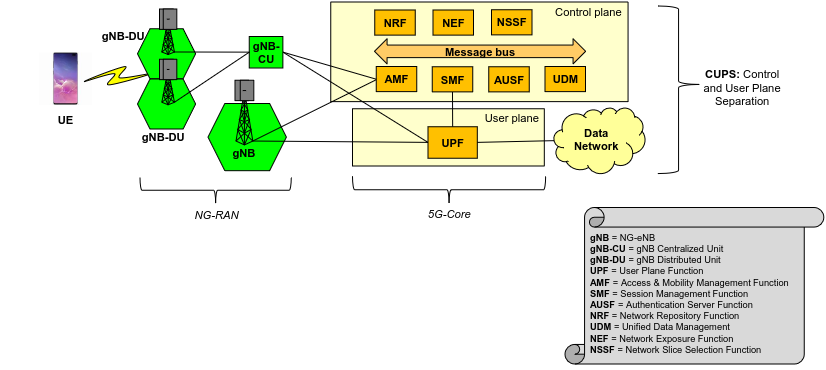
\includegraphics[width=\textwidth]{pictures/12/architettura.png}
	\caption{Architettura del 5G (solo le componenti principali)}
\end{figure}
Tipicamente questa architettura viene chiamata \textbf{Service Based Architecture} (SBA).
Le entità del piano di controllo sono connesse tramite interfacce basate su i servizi (HTTP), tipicamente API RESTful.
\subsection{RAN}
\subsubsection{Next Generation NB (NB)}
Rimpiazza l'attuale eNB (evolved Node B) e ha il compito di gestire le comunicazioni radio con gli utenti attraverso l'interfaccia \textbf{5G New Radio (NR)}.
Può essere disaggregato in due componenti: 
\begin{itemize}
	\item gNB-DU (Distributed Unit): gestisce layer 1 e layer 2 (lower sub layer) del protocollo radio
	\item gNB-CU (Centralized Unit): gestisce layer 2 (higher sub layer) e layer 3 del protocollo radio
\end{itemize}
Un gNB-CU può gestire più gNB-DU, quindi è un buon candidato per la virtualizzazione e per essere posizionato in un cloud. Questo porta al concetto di \textbf{cloud RAN}.
Le gNB-DU possono essere posizionate vicino alle antenne (entro 1ms di latenza).
\subsubsection{SD-RAN}
La RAN può essere implementata secondo il paradigma di SDN, dove gli gNB, gNB-DU e gNB-CU sono controllati da un controller SD-RAN.
Diverse applicazioni possono essere eseguite sul controller SD-RAN, ad esempio per il RAN slicing, handover etc.
\\
\underline{N.B.} C-RAN e SD-RAN sono due approcci ortogonali.
\subsection{Core network}
Ora presentiamo le funzionalità sul piano di controllo e il confronto con la loro controparte nel EPC 4G.
\begin{figure}
	\centering
	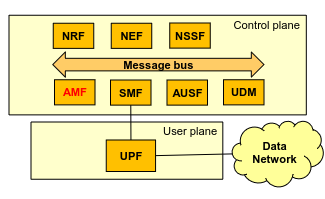
\includegraphics[width=0.5\textwidth]{pictures/12/AMF.png}
	\caption{Componenti principali del piano di controllo del 5G}	
	\end{figure}
\begin{itemize}
	\item \textbf{Access \& Mobility Management Function (AMF)}: gestisce la mobilità tra UE e reti 5G. Gestisce le funzionalità relative alla mobilità del MME del EPC
	\item \textbf{Session Management Function (SMF)}: gestisce le sessioni e l'allocazione degli indirizzi IP. Una sessione in SBA è un'estensione del concetto di bearer in LTE. L'SMF corrisponde alle funzionalità del piano di controllo di MME e SGW/PGW in EPC, relativamente alla gestione di bearer e connettività IP.
	\item \textbf{Authentication Server Function (AUSF)}: gestisce l'autenticazione degli utenti. Corrisponde alle funzionalità di HSS in EPC.
	\item \textbf{Unified Data Management (UDM)}: repository delle informazioni degli utenti iscritti, usato da più funzioni. Analogo a HSS in EPC, ma non effettua autenticazione.
	\item \textbf{Network Repository Function (NRF)}: mantiene informazioni sulle funzioni di rete disponibili. Supporta un meccanismo di discovery per le funzioni.
	\item \textbf{Network Exposure Function (NEF)}: espone in modo sicuro i servizi offerti dalla rete 5g agli utenti (logging, analitiche, etc.). Espone delle API.
	\item \textbf{Network Slice Selection Function (NSSF)}: seleziona la corretta Network Slice Instance (NSI) basandosi sulle informazioni ottenute durante il processo di attach. Redirige quindi il traffico verso la corretta slice.
\end{itemize}
Per quanto riguarda il piano utenti \textbf{User plane Function (UPF)} è responsabile per il routing dei pacchetti e il forwarding tra RAN e reti esterne. Inoltre, mantiene i QoS. Equivale alle funzionalità del piano utenti di PGW e SGW  
\begin{figure}
	\centering
	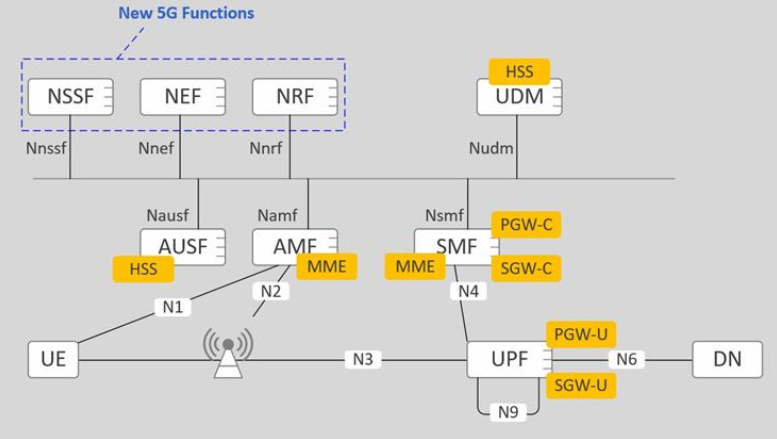
\includegraphics[width=0.7\textwidth]{pictures/12/confronto.png}
	\caption{Confronto tra le funzionalità del piano di controllo del 5G e quelle del EPC 4G}
\end{figure}
\begin{figure}
	\centering
	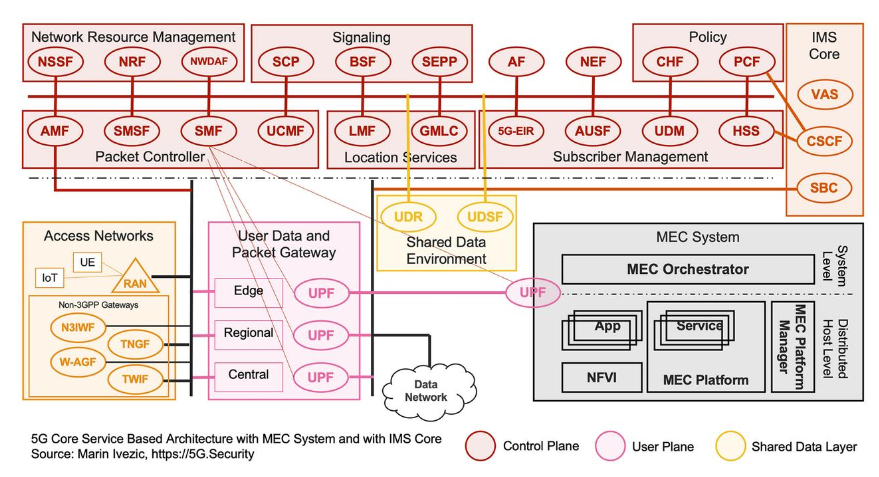
\includegraphics[width=\textwidth]{pictures/12/architetturaSBA.png}
	\caption{Struttura dell'architettura SBA del 5G}
\end{figure}
\section{Transizione da 4G a 5G, deploy}
Ci sono due possibili approcci per la transizione da 4G a 5G immaginati da 3GPP:
\begin{itemize}
	\item Standalone (SA): utilizzo della rete 5G (NG-RAN e 5G-Core) da zero, tenendo separato il 4G.
	\item Non-Standalone (NSA): I nuovi gNB vengono connessi agli EPC 4G (NG-RAN e 4G EPC), la rete core viene evoluta in maniera incrementale verso il 5G-Core.
\end{itemize}
Attualmente la maggior parte dei deploy è basata su NSA. Gli operatori italiani offrono una vasta copertura 5G, concentrandosi principalmente sul garantire alte velocità.
Viene posta poca attenzione verso la latenza e nessun reale interesse nelle densificazione delle celle (small cells, mmWave), che è invece fondamentale per sfruttare appieno le potenzialità del 5G. Al momento non siamo ancora pronti a un deploy completo del 5G, specialmente in Europa. Questo avviene perché a causa dei costi elevati mole funzionalità non verrebbero implementate e l'investimento nelle infrastrutture necessarie è enorme. Per risolvere quest'ultimo problema diversi operatori stanno valutando l'uso d' infrastrutture condivise, sfruttando la virtualizzazione.
\section{Riassunto delle innovazioni}
L'evoluzione portata dal 5G si basa su tre pilastri:
\begin{itemize}
	\item \textbf{Disaggregazione}: split di moduli integrati in modo verticale in funzioni indipendenti.
	\item \textbf{Virtualizzazione}: capacità di far girare delle istanze virtualizzate delle funzioni su hardware di commodity.
	\item \textbf{Commoditization}: capacità di scalare in modo elastico le funzioni in base ai bisogni di carico.
\end{itemize}
Il \textbf{cloud computing} è il paradigma che permette di realizzare queste innovazioni, grazie alla sua capacità di fornire risorse di calcolo, storage e rete in modo dinamico e scalabile. Con 5G il confine tra reti e cloud diventa sempre più labile.